Budujemy nieskończony ciąg figur $\{F_n\}_{n=1}^\infty$.
Figura $F_1$ jest kwadratem o boku długości $a$.
Kolejne figury $F_n$ są budowane z następującą regułą:
\begin{itemize}
    \item Podczas budowy figury $F_{n}$ doklejamy kolejne kwadraty \underline{jedynie} do kwadratów, które zostały dodane w kroku ($n-1$). 
    \item Dzielimy boki $F_{n-1}$ na trzy równe części.
    \item Do środkowej części każego z podzielonych boków doklejamy mniejszy kwadrat o boku długości $a_{n-1}\over 3$
\end{itemize}

\begin{figure}[htbp]
    \centering
    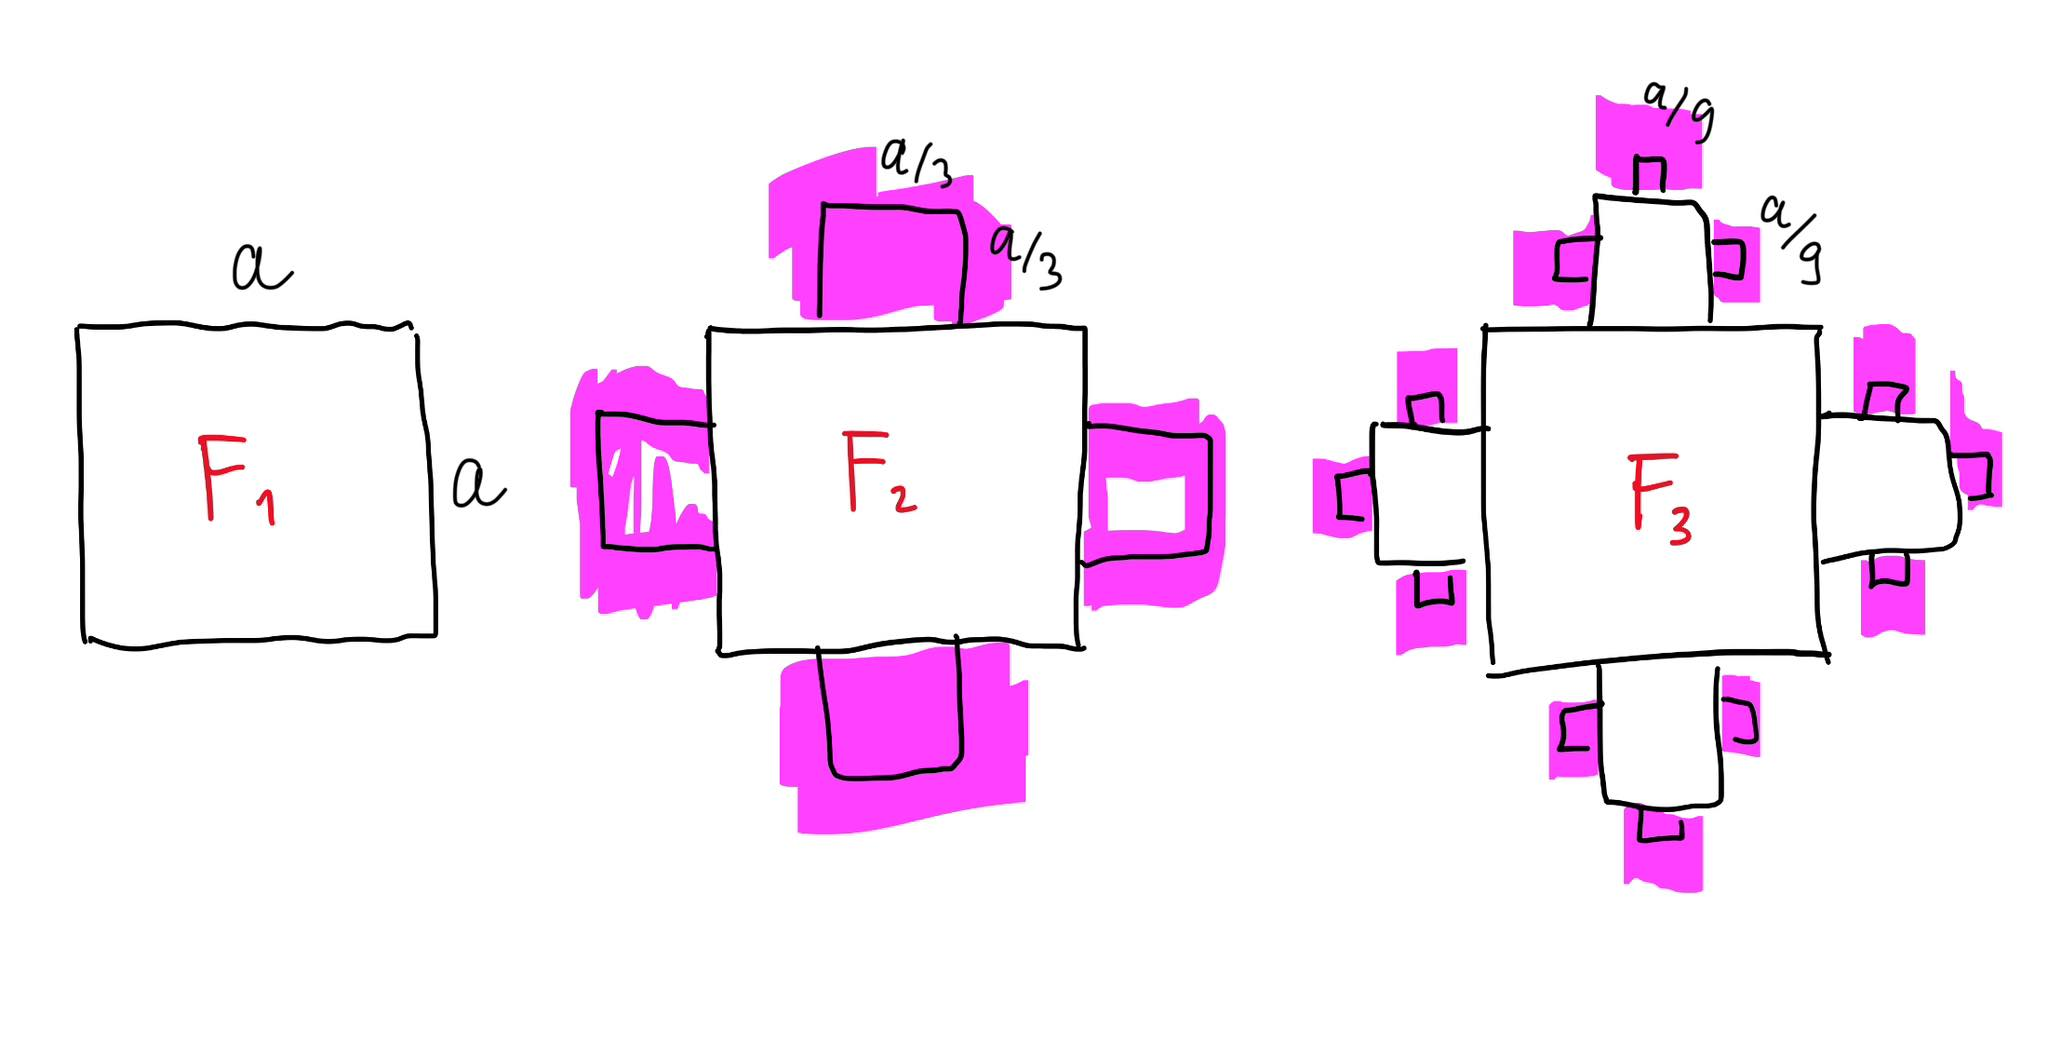
\includegraphics[width=0.6\columnwidth]{figures/zad10.png}
    \label{fig:enter-label}
\end{figure}


\begin{enumerate}
    \item \textbf{Wykaż, że pole figury $F_n$ wyraża się wzorem}:
$$
P_n = a^2\left({5\over 3} - {2 \over {3^n}}\right)
$$
\item \textbf{Oblicz pole figury $F_\infty$ dla wartości $a=3$.}

\end{enumerate}